
\chapter{\uppercase{Model Checking}}
\label{chap:modelchecking}
\graphicspath{{./}{./fig/}{./fig/nimble/}}

It is important to prove the correctness of our algorithms. Specifically, we need to verify the suffix causal consistency property for SCC and the waypoint enforcement property for \sysname. In this chapter, we describe how to use model checking to demonstrate the correctness of SCC and \sysname, respectively. Model-checking tools have long been used to check for violations of network properties and automatically find bugs in network applications.  Recent works~\cite{mcopenflow, flowchecker, nice} use model checking to verify network-wide properties for SDN. It is not easy to do so since these methods need to consider the ample space of switch states and the large space of input packets. An SDN switch maintains a flow table that may store a large number of rules and that processes a packet based on the matching rule of the highest priority. Also, the OpenFlow specification allows switches to match packets to rules based on source and destination IP addresses, source MAC addresses, destination MAC addresses, and specific network protocol.  Though prior works try to address these issues use symbolic execution~\cite{symbolic} or simplified switch and packet models, there are additional challenges that prevent existing tools~\cite{mcopenflow, flowchecker, netplumber, hsa, sdnracer, nice, atpg, veriflow} from being directly applied to our algorithms.
 

First, we need to model unknown delays for each switch update to occur since updates are pushed to switches simultaneously (within a single update step for \sysname). This indicates each switch can possibly have an old or new state depending on the delay during the update. Naively, we can use the model checking tool to explore all possibilities for switch states. However, our SCC algorithm guarantees that, once a packet is matched to a forwarding rule in a switch (i.e., reads a switch state), it can be matched in downstream switches only to rules that are equally or more up-to-date (i.e., it cannot read a stale state for downstream switches). Therefore, we explicitly formulate these constraints to model our algorithms. 

Second, our SCC algorithm needs to compare an extra header field $\pktID{}{\tagTmpField}$ of a packet with $\ruleID{}{\epochField}$ when searching for a matching rule on a switch. This field $\pktID{}{\tagTmpField}$ may be updated by any switch depending on the value of $\ruleID{}{\tagTmpField}$. Also, some rules remain unchanged during the previous configurations and thus $\pktID{}{\tagTmpField}$ can be any value from the range of $[1, \epochField]$. To tackle this, our model adds two fields $\ruleID{}{\epochField}$, $\ruleID{}{\tagTmpField}$ for each rule \ruleID{} and a field $\pktID{}{\tagTmpField}$ for each packet \pktID{}. The model checking tool explores all possibilies for $\pktID{}{\tagTmpField}$ as long as the constraints defined for SCC protocol are satisfied.

Third, \sysname can work with any routing-update algorithm that guarantees relaxed waypoint correctness. The update of switches may be executed in multiple steps and in any order. Therefore, the model checking tool cannot focus on only a specific protocol but needs to model diverse protocol behaviors. Our model should also take into account the behavior of the tunnel protocol since \sysname uses tunnels to redistribute packets from old to new positions of network functions. We formulate the definition of relaxed waypoint correctness, simplify the behavior of tunnels and let the model checking tool explore all possible rule-update schedules. Next, we elaborate on how we formulate our models using Z3Py~\cite{z3py}, a Python API for the Z3 solver~\cite{Z3Solver}, and how we use the Z3 solver to verify the desired property. 




%Most of the existing works~\cite{netplumber, hsa, sdnracer, nice, atpg, veriflow} either cannot support the verification of properties we need (suffix causal consistency and waypoint correctness), or is not efficient enough to explore all possible update schedule for violations. Therefore, we use SMT solver to model the network settings and update-schedule algorithms. 

\section{Model checking for SCC}
We subjected SCC to
model checking to verify its enforcement of suffix causal
  consistency, as well as black-hole freedom and bounded looping.
We constructed our model with ten switches in a mesh topology and with
three flows. The maximum length of each routing path was six
  switches.  Each switch was allowed ten rules
($\setSize{\switchID{\switchIdx}{\ruleSet}} \le 10$), which was
  adequate to accommodate the rules deployed by our algorithm for any
  well-formed routing policy for a system of this size.  Deployed
rules satisfied the constraints of \secref{sec:model:net}; e.g., if
$\ruleID{\ruleIdx}, \ruleID{\ruleIdxAlt} \in
\switchID{\switchIdx}{\ruleSet}$ then
$\ruleID{\ruleIdx}{\priorityField} \neq
\ruleID{\ruleIdxAlt}{\priorityField}$ or
$\ruleID{\ruleIdx}{\coverField} \cap \ruleID{\ruleIdxAlt}{\coverField}
= \emptyset$.  The fields of each rule were unspecified and so
explored by the model checker; in particular, each rule could cover
any number of flows.  Each flow was routed from its ingress to its
egress using normal switch behavior (e.g., a switch matches a packet
to the highest priority rule that covers it).  For each initial
  rule $\ruleID{}$, $\ruleID{}{\epochField}$ and
  $\ruleID{}{\tagTmpField}$ were allowed to range over $\{1, 2, 3\}$
  (explored by the model checker). We modeled the effects of one new
  epoch\footnote{This is reasonable since we require that one epoch's
  rule changes are deployed to the network prior to starting the
  next.} ($\epochIdx = 4$) that implemented some different routing
policy (i.e., at least one flow traveled a different
path to its egress) using rules for which \ruleID{}{\epochField} and
\ruleID{}{\tagTmpField} were set according to our algorithm.

Z3 explored all possibilities for each new rule and, so, for the
  new path traversed by each flow, constrained only so that each flow's
  ingress was unchanged.  To model unknown delays for switch updates
to occur, each switch that had not yet applied a new rule to a packet
could apply either an old rule \ruleID{1} or new rule \ruleID{2} to
match the current packet \pktID{}, according to
\pktID{}{\tagTmpField}.  Specifically, if $\pktID{}{\tagTmpField} \le
\ruleID{1}{\epochField}$ and $\pktID{}{\tagTmpField} \le
\ruleID{2}{\epochField}$, either rule could be applied to the packet,
creating two branches. If $\pktID{}{\tagTmpField} >
\ruleID{1}{\epochField}$ and $\pktID{}{\tagTmpField} \le
\ruleID{2}{\epochField}$, then only the new rule $\ruleID{2}$ could be
used to match the packet.

To test black-hole freedom, we set a condition that the trace of
each packet should end with the egress node for the packet. The
bounded looping property was defined to require that any unordered
pair of switches cannot occur in the trace more than twice.
The suffix causal consistency property was modeled to require
  that, once a packet arrives at a switch belonging to its new path
  but not its old path, it stays on the new path.
We let the Z3 solver explore all possible switch configurations to
check for violations of these properties.  In previous, incomplete
versions of our algorithm, this model checking revealed corner cases
that we had failed to consider and that resulted in property
violations; several of these corner cases were used in the examples
given in \secref{sec:algo:controller} to motivate the algorithm
stages.  For the algorithm presented in \secref{sec:algo:controller},
however, after running about $6$ days, the model checker successfully 
terminated and found no violations.



\section{Model Checking for Nimble}
\label{sec:schedule:model_checking}

We subjected our algorithm of \secref{sec:migration} to model checking to verify its enforcement of
waypoint correctness described in \secref{sec:goals:correctness}.
We constructed our model with fifteen switches in a mesh topology and
with three flows.  Each routing path was eight switches and each path
contained three NFs.  We modeled the effects of one new epoch that
implemented a routing policy with NF migration (i.e., each network
function for each flow was moved to a different position) using rules
in the old and new configuration.

The underlying route-update algorithm deployed rule updates on
switches (i.e., deleting unused rules and installing new rules) in at
most $\updateSteps = 15$ steps, with each switch being updated at most
once.  Each switch utilized either old or new rules to process packets
based on the step during which it received those packets. For example,
if \switchID{1} was scheduled to be updated in step \updateID{3},
\switchID{1} used an old rule \ruleID{1} to match \flowID{1} before
\updateID{3} began and a new rule \ruleID{2} after \updateID{3}
completed.  During \updateID{3}, to model unknown delays for switch
updates to occur, either \ruleID{1} or \ruleID{2} was used to match
\flowID{1} nondeterministically. The step at which packets were
received by each switch through the network was non-decreasing.
Moreover, the update schedule generated by the underlying route-update
algorithm ensured relaxed waypoint correctness.  Z3 explored all
possible rule-update schedules constrained by the above conditions to
enforce new routing policy of each flow.  As such, the model checked
was not dependent on any specific route-update protocol, but rather
permitted any route-update strategy as long as it satisfied these
properties.

Our algorithm incorporated NF migration into the rule-update schedule
generated by the underlying route-update algorithm and used tunnels to
redistribute packets from old NF locations to new ones. For
simplicity, the correctness of tunnels was assumed, and tunnels were
not modeled explicitly.  Specifically, when a packet on flow \flowID{}
arrived at \oldSwitchID{\nfIdx} and was matched to rule
\ruleIDIn{\nfIdx}, the packet was delivered to \newSwitchID{\nfIdx},
as if through the tunnel.

To model the delay caused by buffering packets at new NF locations,
the specific step at which \newSwitchID{\nfIdx} forwarded packets
using its new rule should not be earlier than the step at which
\newSwitchID{\nfIdx}{\release{\nfIdx}} is invoked. For example, if a
packet arrived at \oldSwitchID{\nfIdx} for \nfID{\nfIdx} at step
\updateID{3} and then was forwarded through the tunnel to
\newSwitchID{\nfIdx}, \newSwitchID{\nfIdx} could not release packets
until \newSwitchID{\nfIdx}{\release{\nfIdx}} was deployed at step
\updateID{5}. We let the Z3 solver explore all possible delays before
the \newSwitchID{\nfIdx} released packets and check for violations of
waypoint correctness as defined in \secref{sec:goals:correctness}.  In
previous, incorrect versions of our algorithm, this model checking
revealed corner cases that we had failed to consider and that resulted
in property violations.  For the algorithm presented in the previous
sections, however, after running about one day on a 32-core,
2.1\gigahertz computer with 256\gigabytes of memory, the model checker
successfully terminated and found no violations.

\iffalse
\liu{I am not sure if we need this counterexample. It is quite artificial. Just leave here in case you are interested.}
It is hard to determine the time for the controller to deploy \newSwitchID{\nfIdx}{\release{\nfIdx}} on \newSwitchID{\nfIdx} to release packets buffered by \nfID{\nfIdx}.
\mkr{The algorithm in \secref{sec:migration} adds these invocations
  to \updateID{\updateSteps+1}.  Is that wrong?}
In most cases, the controller can send releasing command at step when rule update is scheduled for \newSwitchID{\nfIdx} if the tunnel has been built, since the rule deployment on \newSwitchID{\nfIdx} usually means the downstream switches have been updated and the new forwarding rule on \newSwitchID{\nfIdx} is ready to use. However, our model checking found a counter example shown in \figref{fig:counterexample}. Assume the path of packets was changed from $\switchID{1} \rightarrow \switchID{2} \rightarrow \switchID{3}$ (solid line) to $\switchID{1} \rightarrow \switchID{4} \rightarrow \switchID{5} \rightarrow \switchID{6} \rightarrow \switchID{3}$ (dash line). \nfID{1} was migrated from \switchID{2} to \switchID{4}. The underlying route-update algorithm generated the following rule-update schedule for the path change. The controller updated \switchID{6} and built a tunnel between \switchID{2} and \switchID{4} at step $1$, and then installed forwarding rule on \switchID{4} at step $2$ before updating \switchID{6} at step $3$ and \switchID{5} at step $4$. At last, \switchID{2} was updated to forward packets through the new path so that packets traversed either old or new path. If \switchID{2} received \ruleIDIn{2} at step $2$ and \switchID{4} received \switchID{4}{\release{\nfIdx}} to release packets at step $3$. Packets were dropped on \switchID{5} since it did not have a new rule yet. Therefore, packets can only be released by \newSwitchID{\nfIdx} when \newSwitchID{\nfIdx} starts to receive packets sent from the upstream switch (not through the tunnel).  
\mkr{We should discuss this.  Are you saying that we need to change the
  semantics of the release command?} \liu{This should be an example motivating "update schedule" step in our algorithm.}

\begin{figure}
\centering
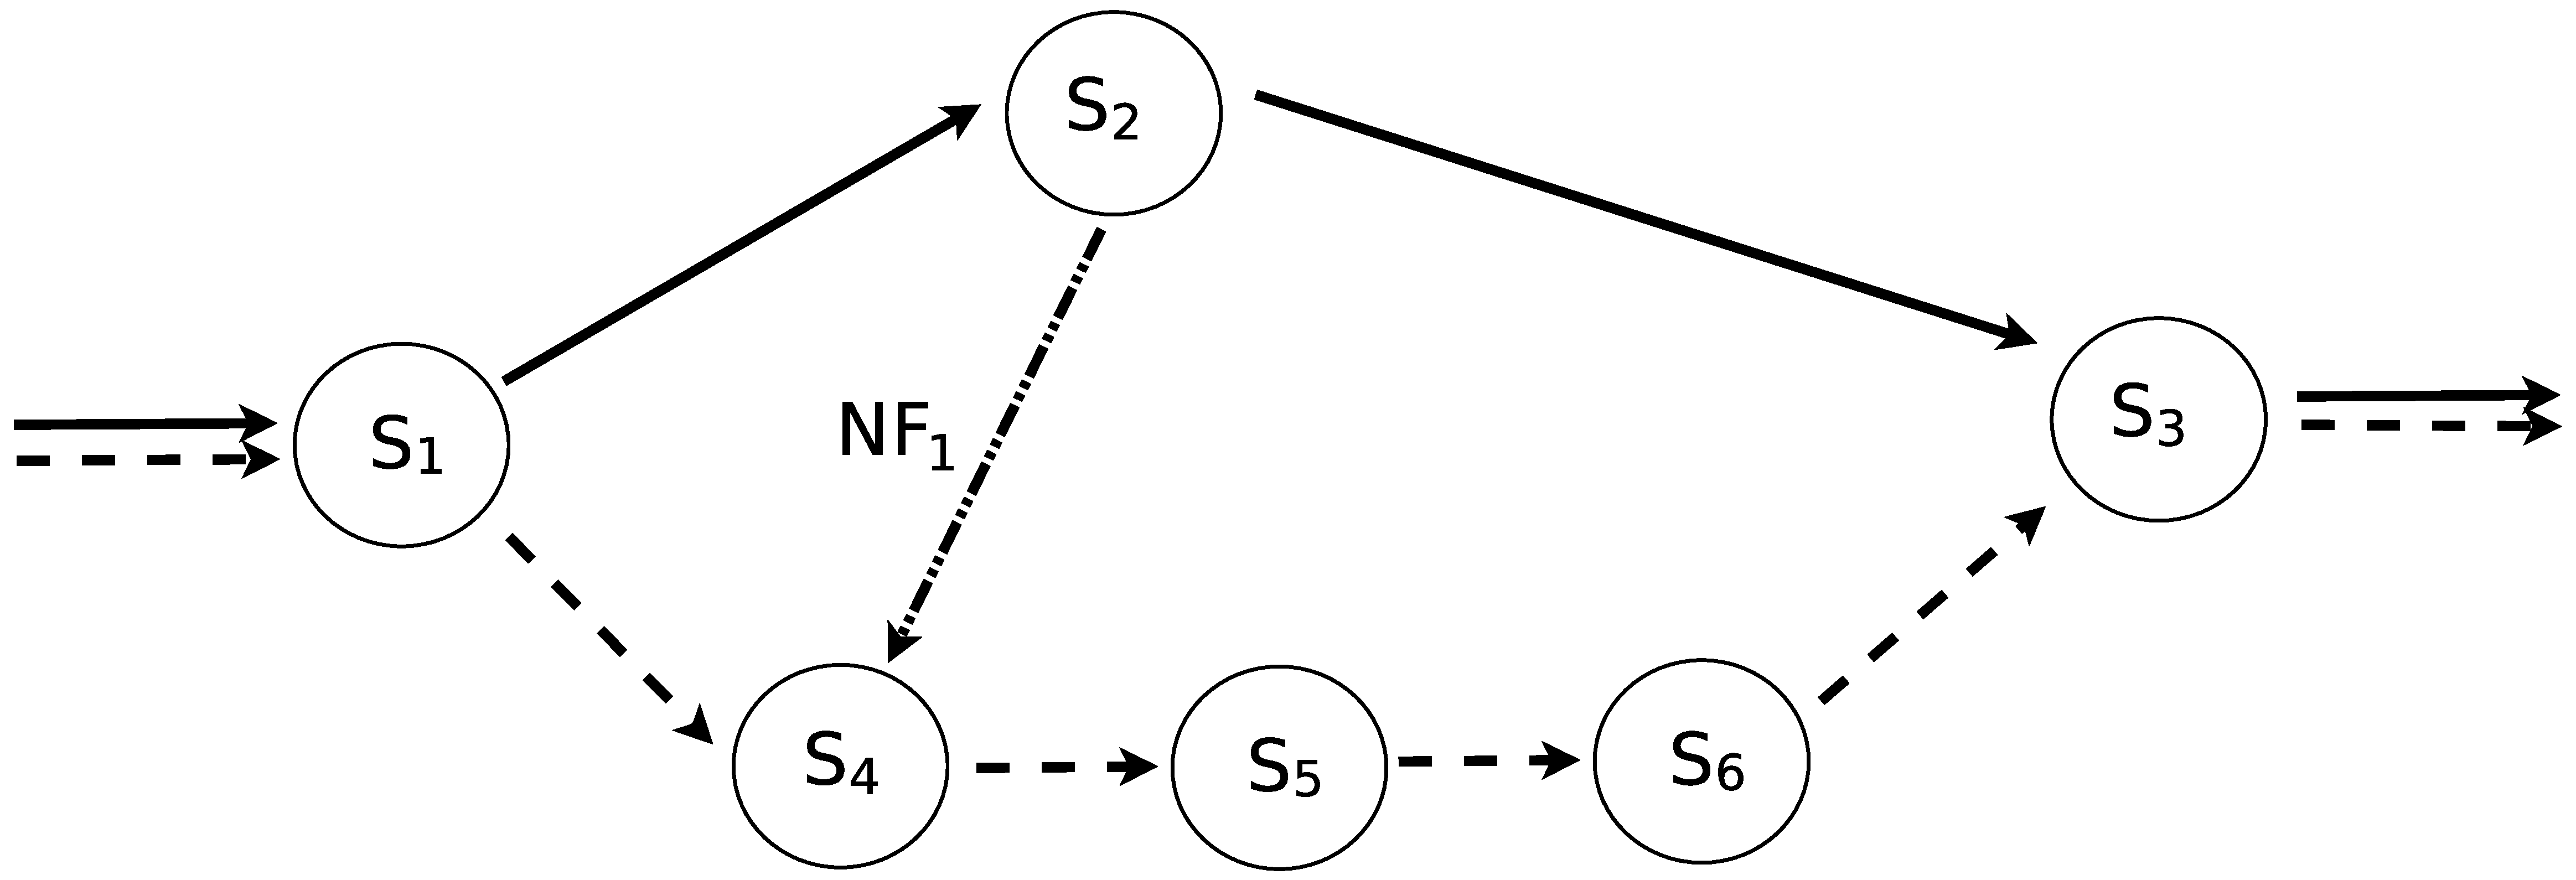
\includegraphics[width=0.45\textwidth]{counterexample.eps}
\vspace{-0.3cm}
\caption{Counterexample for model checking}
\label{fig:counterexample}
\vspace{-0.5cm}
\end{figure}
\fi
